\section{Evaluation}
\label{sect:apner_results}
We first report on a study in which we evaluate the generation of candidates entities using the vector similarity measures and representative (commonly used) entities. 
%\logan{Would using "candidate entities" rather than "distance candidates" make more sense?}
%\logan{If F\ref{fig:current} describes your setup. Why not reference it here?}\roselyne{That is the set up for the active learning but I also evaluate the candidate generation, so I think for now, I'll leave it out but see if I refer to it in the sections below.}
We then discuss the results of initial classification and subsequent four rounds of active learning using multiple word vector classifiers and our three sampling strategies: random, UBS, and Distance UBS.
Finally, we experiment with word representations enhanced with character-level information using FastText~\cite{bojanowski2016enriching,joulin2016bag}.

\subsection{Dataset}
We work with a corpus of \num{1690} full-text publications in HTML format from \textit{Macromolecules}, 
a relevant journal in polymer science.
These documents comprise \num{381947} sentences and \num{9229417} (\num{253195} unique) words or ``tokens,''
of which \num{99999}\ian{to be defined} pass the NLP filter of Section~\ref{sec:filter}.

From this corpus, 
we set aside a test set of 100 documents with  \num{22664} sentences and \num{508391} (\num{36293} unique) tokens,
of which \num{9656} pass the NLP filter.
We engaged six experts to identify all one-word polymer names in this test set,
a process that produced 467 unique one-word polymer names.
We use these 467 names as a gold standard in subsequent subsections.
%When testing against this gold standard, 
%we evaluate using a total of \num{9656} NLP-filtered nouns from the 100 documents.

\ian{Seems odd to have the following text in a subsection on ``Dataset.'' Maybe move to start of this section?}
We evaluate extraction accuracy in terms of precision and recall.
Recall refers to the fraction of actual positives that
are labeled correctly and precision to the fraction of predicted
positives that labeled correctly.
%\logan{What part of this data can we release, if any?}\roselyne{Hong and I are working on a dataset following a schema we discussed for release, I think we talked about it but didn't update you guys back. However it's more like NLP datasets, where we are releasing sentences with entities and not this exact dataset}

\subsection{Word Embedding Settings}
\ian{Are you exploring these issues in general, as the first sentence states, 
or are you trying to find good values for these settings, for use in subsequent work? I can't tell.}
%\logan{Needs better topic sentence. Say why you are doing this more clearly, less about the "what"}
In order to maximize the number of actual entities in the dataset\textemdash and the ratio of target to non-target entities\textemdash in the initial set of labels,
we explore how the choice of seed entities and the internal parameters \texttt{vector} and \texttt{window_size} impact the number of target entities retrieved using similarity measures.

\ian{Maybe the following would be simpler if written as follows. This seems to say what you are trying to say?: 
``We use the 467 gold standard polymer names identified by experts in our 100-document test set to
evaluate the performance of different word embedding settings.
Specifically, for each choice of settings that we want to evaluate,
we determine the \num{10000} distance candidate vectors that are most similar to the representative entity vectors 
and report what fraction of the 467 gold standard names are included in that \num{10000}.
We use lower-case exact string matching between the gold standard polymer names and the proposed distance candidate strings to determine if a candidate is a polymer.}

To estimate the entity-richness of our large pool of distance candidates and since we do not have manually extracted data for the entire corpus, we create a list of \num{10000} distance candidate vectors most similar to our representative entity vectors and report the fraction of gold standard polymers extracted. 
In our gold-standard of publications, there are $\sim$5 polymers per document (\num{8450} polymers for \num{1690} documents). Thus, we expect a fraction of the polymers found in the 100 gold standard documents to be extracted in the \num{10000} candidates most similar to our seed entities.
\ian{I have no idea what you are trying to say here $\ddot\smile$. You say ... ``our gold-standard of publications ... 1690 documents'', but previously you define the gold standard as being 100 documents.}
%\logan{This is confusing. Why are we using a model to estimate the total population of the polymers and not just assuming the gold-standard is a representative sample?}\roselyne{ok, 467/100)}
We evaluate the entity-richness of polymers in this pool of candidates by measuring the percentage of the 467 manually extracted polymer names that it yields;
we use lower-case exact string matching between the gold standard polymer names and the proposed distance candidate strings to determine if a candidate is a polymer.
\roselyne{Since I removed parameter tuning, add choices of parameters here?}

\subsubsection{Representative Candidates}
Here, we focus on how the choice of seed entities affects the fraction of polymers in the candidates, which we take as a measure of the entity-richness of the pool of candidates.
%\logan{This is confusing. Is the fraction of polymers in the candidate pool not the recall?}\roselyne{yes, why? I've replaced the word recall.}
In previous work using the same corpus~\cite{tchoua2016hybrid,tchoua2016hybridi}, we build a dictionary of polymer names by using a rule-based approach and aggregating synonyms across ChemDataExtractor records. (A record consists of all information found about a chemical entity in a document.)  
Here we use this dictionary to identify the 10 most frequently occurring polymers in our corpus and their acronyms.
%Experts can also suggest these entities based on prior knowledge.
We assume that frequent polymers provide a large number of example sentences that illustrate context in which polymers are commonly used.
%\logan{Do you think it would be better to use the gold standard, where we have certainty of the labels, to estimate the most-frequent polymers?}\roselyne{we used the entire corpus, we know the most frequent polymers}
Hence, we first test the most common, the three most common, and the ten most common polymers as seed entities.
%\logan{The circularness of this strategy makes me uncomfortable. We use an NER model to determine the initial training set for the NER model? How would you address this criticism?}\roselyne{not sure I understand how I am using an NER model to determine the NER model, I'm just testing with various seed entities. As you suggested before, experts can give this info, or we can just measure the frequency of a few known entities. Added a line about this so that no prior work is needed.}
We experiment with including and excluding their acronyms as additional seed entities.
(Note that this modest set of 1, 3 and 10 seed entities could also be suggested by an expert.)
Rows 1--6 of Table~\ref{tab:candidate_generation} shows the results for this set of experiments.
When using \textit{polystyrene} (the most commonly used name) as a seed entity, the pool of candidates contained 33.55\% of the 467 gold standard polymers.
%\logan{Another potential criticism: Would I need a gold standard to build the NER method? I thought your method is supposed to help me avoid having to do the work for generating a gold standard?}\roselyne{There is no way to evaluate if you don't have a gold standard is there?}
We note a 2\% increase in the fraction of polymers retrieved when using \textit{polystyrene} and its acronym compared to using \textit{polystyrene} alone.% (37.69\%).
%\logan{Is this an important detail? Why does it need to stay [I think this section is a little dense]}\roselyne{well, before Kyle thought this was a bit vague, so I added lots of numbers, I may come back and remove this}\roselyne{Removing details from here}
The fraction of polymers increases by 10\% when using the three most frequent polymers as representative entities; %(from 33.55\% to 46.9\% and 47.97\% with acronyms); 
the three most frequent polymers in our datasets are \textit{polystyrene},\textit{poly(methyl methacrylate)},\textit{polyethylene}.% and their acronyms (\textit{PS}, \textit{PMMA} and \textit{PE})
Using ten instead of three entities however, only slightly increases the yield of polymers by less than 1\%.%, from 47.97\% for three frequent polymers with acronyms to 48.39\% for ten frequent polymers with acronyms.

\begin{table}[ht!]
\centering
\caption{Fraction of gold standard polymer names extracted from pool of \num{10000} \textit{distance} candidates with different candidate generation methods.\label{tab:candidate_generation}\ian{I don'tt hink it is credible to have four significant figures given that there are only 467 gold standard names. Three is plenty.}
}
\vspace{2ex}
%[35.55, 37.69, 46.9, 47.97, 46.47, 48.39, 46.68, 36.4]
\setlength\tabcolsep{3pt}
\begin{tabular}{|C{0.1in}|C{2.4in}|C{0.6in}|}
 \hline
\textbf{\#} & \textbf{Candidate Generation Method} & \textbf{Fraction of polymers extracted}  \\
\end{tabular}
\begin{tabular}{|C{0.1in}|R{2.4in}|L{0.6in}|}
\hline
 1 &    Polystyrene & 35.55\%  \\
\hline
 2 &    Polystyrene with acronym (PS) & 37.69\%\\
\hline
 3 &    3 most frequent polymer names & 46.90\%\\
\hline
 4 &    3 most frequent polymer names with acronyms &  47.97\%\\
\hline
 5 &    10 most frequent polymer names & 46.47\%\\
\hline
 6 &    10 most frequent polymer names with acronyms & 48.39\%\\
\hline
 7 &    $\chi$DB polymer names & 46.68\%\\
\hline
  8 &  crowDB polymer names    & 36.40\%\\
\hline
\end{tabular}
\end{table}

In a second set of experiments, we explore the idea of using larger numbers of seed entities to increase the fraction of polymers retrieved in the pool of candidates.
We have built a small database of polymer properties ($\chi$DB) in previous work~\cite{tchoua2016hybrid,tchoua2016hybridi}. 
Our corpus of \num{1690} publications included 111 our of 175 $\chi$DB polymers.  
We also scraped CrowDB, which lists some polymers and their properties at \url{http://polymerdatabase.com/} for polymer names.
In this case, 32 out of 295 scraped polymer names were found in our corpus.
We experiment using these 111 and 32 seed entities to extract polymers. The fraction of polymers from our gold standard is shown on rows seven and eight in Table~\ref{tab:candidate_generation}.
These results confirm using more entities does not increase the yield of polymers, as some polymers have low frequency in the corpus, words that are most similar are less likely to be targets.
For the remainder of the experiments, we use the three most frequent polymers and their acronyms. 
%\logan{I think the metric we use for choosing an algorithm here (fraction of entries in the training set) is too indirect. Why not use the performance of the initial ML model to rate how good the training set is? A hypothetical concern with the metric as well: Does your current metric mean a pool with 100\% polymers would be the best? Wouldn't that lead to the same problem of imbalance as having no polymers?}
%\roselyne{how about just 50-50\% what would be wrong with training on such a dataset, why should we reach 100\%, maybe I should add somewhere that this is a good ration, or anywhere higher than 10\%. I will consider that next time, but I think this made sense to me, increase from 5\% to reduce imbalance. I mentioned in the discussion that we evaluated based on entity richness but could evaluate in terms of discrimination, it's a lesson learned.}


%\kyle{perhaps better as a table. The long labels are hard to read}\roselyne{ok}
%\begin{figure*}
%\centering
%\begin{minipage}[b]{.4\textwidth}
%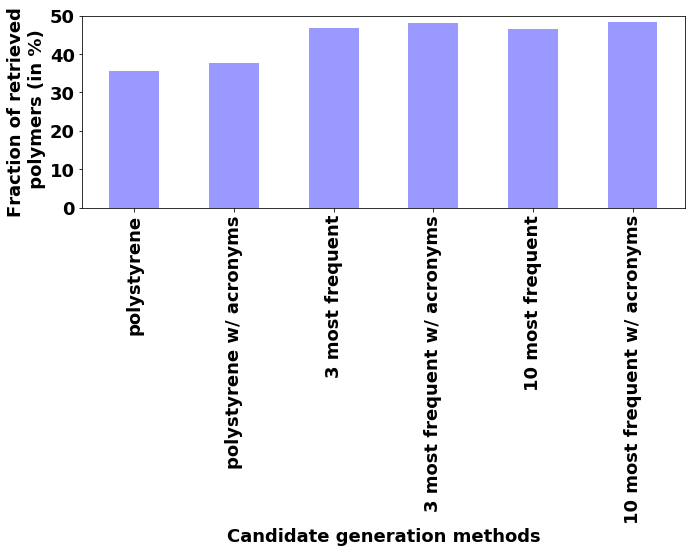
\includegraphics[trim=0in 0.1in 0.1in 0.in,clip,width=1.0\textwidth]{figures/candidate_generation_method1.png}
%\caption{\label{fig:cand_generation1} Fraction of polymer retrieved for various candidate generation methods using most common, three most common and ten most common polymer names as seed entities.
%}
%\end{minipage}\qquad
%\begin{minipage}[b]{.4\textwidth}
%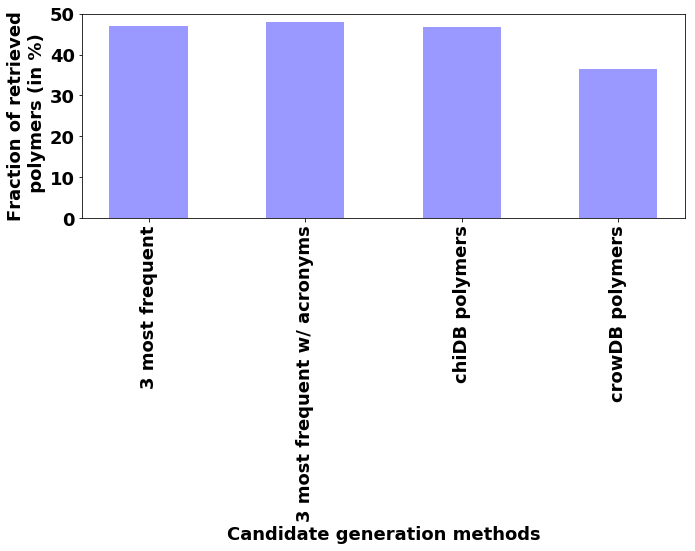
\includegraphics[trim=0in 0.1in 0.1in 0.in,clip,width=1.0\textwidth]{figures/candidate_generation_method2.png}
%\caption{\label{fig:cand_generation2} Fraction of polymer retrieved for various candidate generation methods using three most common (with and without acronymss), $\chi$DB and CrowDB polymer names as seed entities.  
%%\kyle{Not sure this needs to be a separate graph?}
%}
%\end{minipage}
%\end{figure*}
%Together
%[35.55, 37.69, 46.9, 47.97, 46.47, 48.39, 46.68, 36.4]
%[35.55, 37.69, 46.9, 47.97, 46.47, 48.39]
%\begin{figure}[!t]
%\centering
%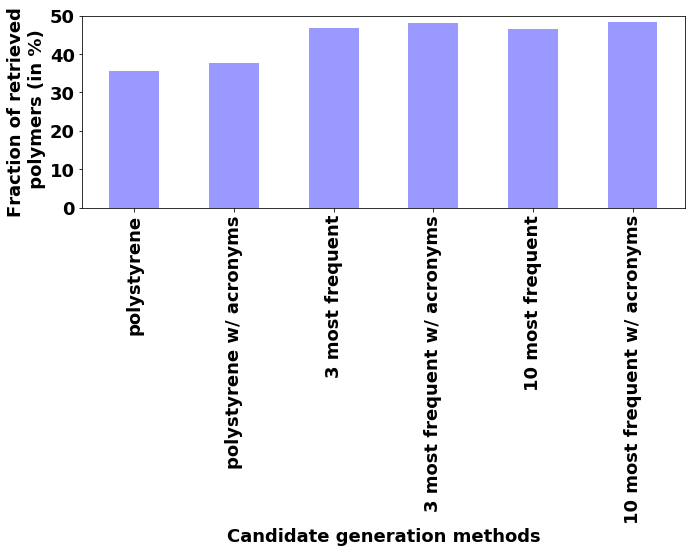
\includegraphics[trim=0in 0.1in 0.1in 0.in,clip,width=3.5in]{figures/candidate_generation_method1.png}
%\caption{\label{fig:cand_generation1} First set of experiments with seed entities showing noticeable improvement from 1 to 3 and less improvement from 3 to 10 seed entities.
%}
%\end{figure}
%[46.9, 47.97, 46.68, 36.4]
%\begin{figure}
%\centering
%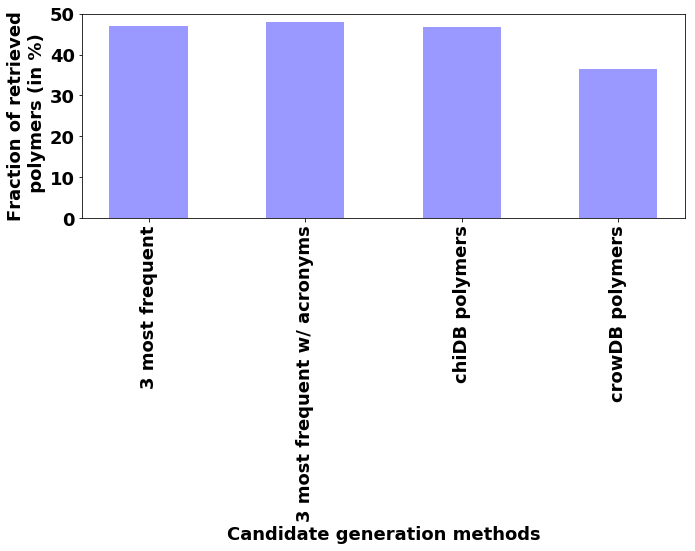
\includegraphics[trim=0in 0.1in 0.1in 0.in,clip,width=3.5in]{figures/candidate_generation_method2.png}
%\caption{\label{fig:cand_generation2} First set of experiments with seed entities showing that using more polymers as seed entities does not necessarily enrich the pool of distance candidates.
%}
%\end{figure}

%\subsubsection{Word Embedding Window and Size Parameters}
%We generate a pool of \num{10000} candidates most similar to the three most frequent polymers and their acronyms from a test corpus of \num{1690}, excluding any token found in our test documents. 
%As previously mentioned, to measure the entity-richness of our dataset, we compute the fraction of polymers retrieved using the similarity measure to our representative entities in the  \num{10000} candidates.
%%We measure the impact of the \textit{window} and \textit{size} on the fraction of polymers extracted from the gold standard in the list of \num{10000} candidates most similar to our representative entities. 
%%\logan{Where are the 10k candidates from again? Could we reference this set by its purpose rather than its size?}\roselyne{Done I think.}
%%\logan{Need a reason why this is important? Also, this statement again raises my concern about using "fraction extracted from gold standard" as a metric for quality of the initial training set?}\roselyne{same answer as above, trying to increase balance in dataset.}
%The \textit{window} represents the maximum distance between the current and predicted word within a sentence. In other words, it represents the number of words before and after each word considered by the neural network to generate a vector representation for that word. 
%For each parameter setting, we measure the yield of polymers ten times for each window and vector size setting.
%We observe slightly higher fraction of polymers retrieved for window sizes of 1 and 2. The yield subsequently decreases and more noticeably with window size larger than 5 (see Figure~\ref{fig:window_size}).
%The \textit{size} determines the size of the word vector (features for our classifier).
%We varied this parameter between 100 and 500.
%The average yield of polymer names was measured at 49.3 with a standard deviation of less than 1\% (see Figure~\ref{fig:vector_size}).
%We conclude that the vector size does not impact the fraction of polymers retrieved during the distance candidate generation.
%[49.67880085653105, 49.25053533190578, 49.46466809421842, 49.46466809421842, 48.82226980728051]
%\logan{Need a concluding sentence?}


%\begin{figure}
%\centering
%%\begin{minipage}[b]{.4\textwidth}
%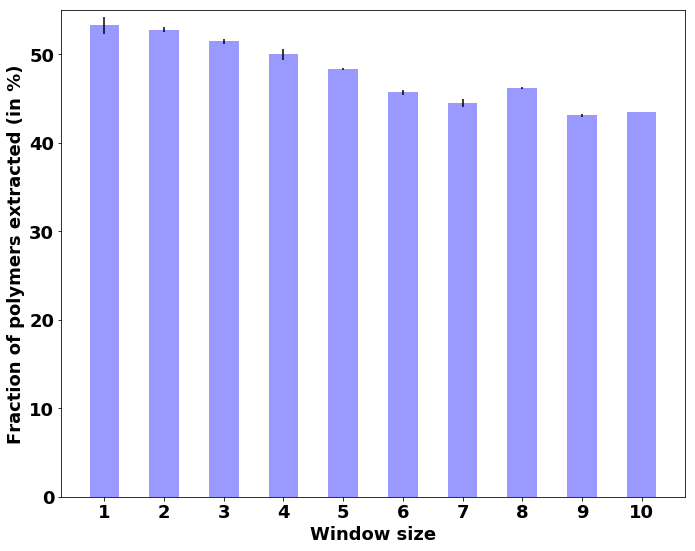
\includegraphics[trim=0in 0.1in 0.1in 0.in,clip,width=3.5in,height=2.5in]{figures/window_size.png}
%\caption{Impact of varying window size on fraction of polymers retrieved.}\label{fig:window_size}
%%\end{minipage}\qquad
%%\begin{minipage}[b]{.4\textwidth}
%%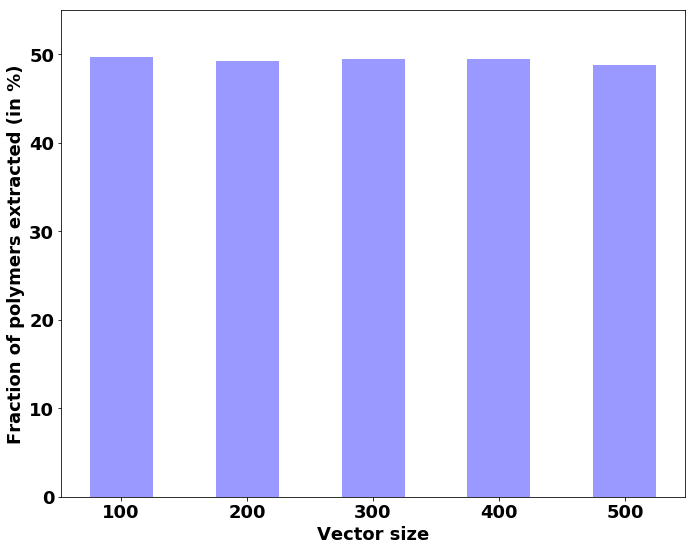
\includegraphics[trim=0in 0.1in 0.1in 0.in,clip,width=1.0\textwidth]{figures/vector_size.png}
%%\caption{Impact of varying vector size on fraction of polymers retrieved. \logan{Can we combine this with F\ref{fig:window_size}? (If we keep it) }}\label{fig:vector_size}
%%\end{minipage}
%\end{figure}
 %\kyle{Not sure this fig is worth including}\roselyne{Agreed that it's not so interesting but i think it goes with the windows one and i will combine the two figures you think should be together.}\roselyne{May remove as paper gets longer}

\subsubsection{Initial Classifier}
%Having explored the parameters for distance candidate generation, we generate a pool of \num{10000} candidates most similar to the three most frequent polymers and their acronyms from a test corpus of \num{1690}, excluding any token found in our test documents. 
%\logan{Is the 10k entries mentioned in the previous section this set? If so, we need to revise the order of these sections?}

\ian{Can this be reworded to ``We train the initial classifier on the 200 entities in the previously discussed list of
\num{10000} candidates that have the highest similarity scores.''}
\ian{Then to be consistent, refer to parameters by names as above:
``parameter values  \texttt{vector}=200 and \texttt{window\_size}=2.'' Remind the reader what these parameters are used for?}

We arranged the previous list of \num{10000} candidates in decreasing order of similarity scores.
We train the initial classifier using the first
200 entities from this list.
Recall that the batch size of 200 was set based on an estimate of 30--60 minutes of expert time.\ian{You previously said 60 minutes. Be consistent.}
%\logan{Maybe we can be specific here about how much time it took. "We found that a batch of 200 required ..."}\roselyne{this is an average based on your estimate, but I don't have an exact number from the first test}
As described on Figure~\ref{fig:current}, in the first step, we train and test on candidates generated from a word embedding model generated using only the training documents. 
We train the classifier on 80\% of the data and test on 20\%.

We observe a better-than-random behavior on the Receiver Operating Characteristic (ROC) curve with an AUC of 0.62 as shown on 
Figure~\ref{fig:roc_init}. %shows the Receiver Operating Characteristic (ROC) curve for the initial classifier with highest recall when evaluating on the test corpus.
%\logan{I do not like this as a topic sentence because it doesn't offer any indication of what to draw from the figure. I prefer ones that are "We found that X, as shown in Figure Y." Topic sentences with some editorial comments worked in help keep the narrative of the purpose of your study alive.}
%The ROC plot is an evaluation measure that is based on two basic evaluation measures: specificity (true positive rate) and sensitivity (true negative rate).
%Sensitivity is the same as recall. Specificity is a measure of the true negative rate (the proportion of actual negatives that are correctly identified as such).
%A classifier with the random performance level always has the same true positive rate and false negative rate.
%%\logan{Not true. The TPR depends on how many points you sample, and is always equal to the FPR}\roselyne{oh right.}
%A classifier with the perfect performance level shows a combination of two straight lines immediately showing a true positive rate of 1.0 and remaining there as recall increases.
%Classifiers with better-than-random performance levels usually lie in the area between the random ROC curve (baseline) and the perfect ROC curve.
%\logan{Also not quite correct. All classifiers with better-than-random performance lie between random and perfect. Maybe just skip the notion of betweenness and talk about the AUC}\roselyne{this is what I tried to say, you don't like the word meaningful? I meant if it's below it's usually bad.}
%The area under the curve (AUC) measures the area under the ROC.
%Ideally the AUC of a learning algorithm is above 0.5. 
The AUC can be misleading for imbalanced dataset as it takes into account true negatives or correctly predicted non-polymers (inverse ratio).
For example if a dataset contains 90\% of sample A and 10\% of sample B, if a classifier predicts every sample as belonging to the first class (A), the accuracy reported will be of 90\% but this classifier is not useful in practice.
%Since AUC takes into account true negatives or correctly predicted non-polymers and our dataset is imbalanced containing more non-polymers than polymers, 
Therefore, we also plot the Precision Recall (PR) curve to visualize the tradeoff between precision and recall.%\logan{A little wordy, can you streamline this sentence?}
%\logan{This paragraph contains no conclusions, it just explains the ROC. Add something about the results.}\roselyne{I explain below? will elaborate}
While the AUC for the initial base KNN classifier is above random performance (0.5) in Figure~\ref{fig:roc_init}, the initial PRC shows poor precision regardless of recall (see Figure~\ref{fig:prc_init}).
We have obtained better performance with more labels (897) in our previous implementation~\cite{tchoua2019polyner}, these preliminary results point to the fact that the classifier is beginning to learn but 80\% of 200 labels is not have enough training data to perform well in practice yet.
%\logan{Better topic sentence. It provides a hit of what to look for. But, you do not follow it up with any details supporting this claim}\roselyne{yes this is where i was doing some explaining for the paragraph, will elabotate}
%\logan{This is a long section for just describing how you made the classifier and that it is pretty bad. Do we need this section?}\roselyne{I will shorten and improve next, the main reason for poor performance is small sample data, because we know this works better with 800 data points, from previous polyNER paper.}

\ian{Presumably you will fix the layout and figure labels for Figs~\ref{fig:prc_init} etc.}

\ian{You refer in different places to ``Receiver Operating Characteristic Curve," ``Receiver Operating Curve,''
and Receiver Operation Curve.'' I changed all to ROC curve to be consistent.}

\begin{figure*}
\centering
\begin{minipage}[b]{.4\textwidth}
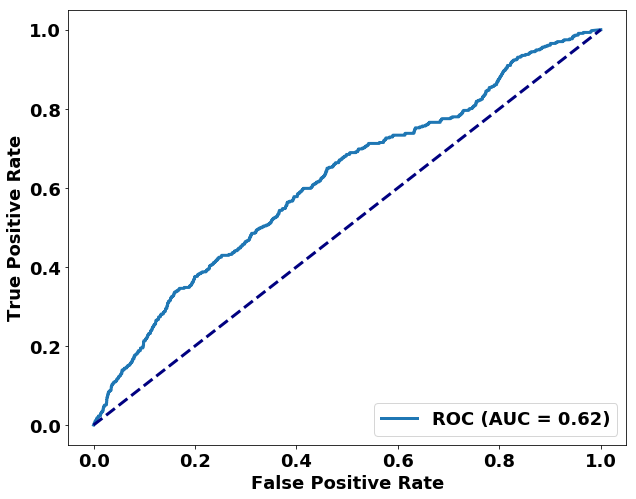
\includegraphics[trim=0in 0.1in 0.1in 0.in,clip,width=1.0\textwidth]{figures/roc_init.png}
\caption{ROC curve for KNN model for initial round of labels.}\label{fig:roc_init}
\end{minipage}\qquad
\begin{minipage}[b]{.4\textwidth}
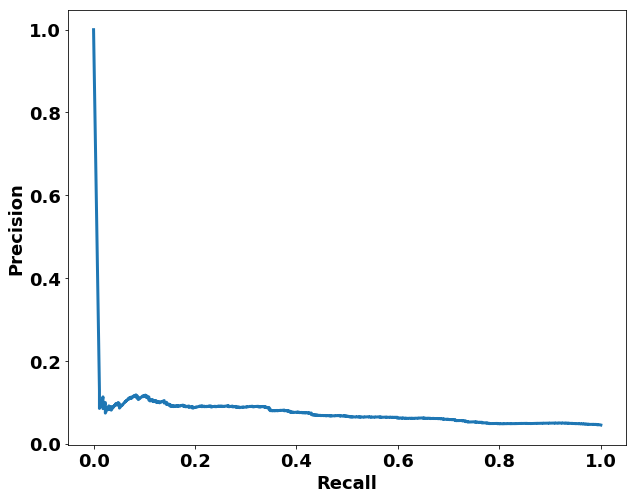
\includegraphics[trim=0in 0.1in 0.1in 0.in,clip,width=1.0\textwidth]{figures/prc_init.png}
\caption{PR curve for KNN model for initial round of labels.}\label{fig:prc_init}
\end{minipage}

\centering
\begin{minipage}[b]{.4\textwidth}
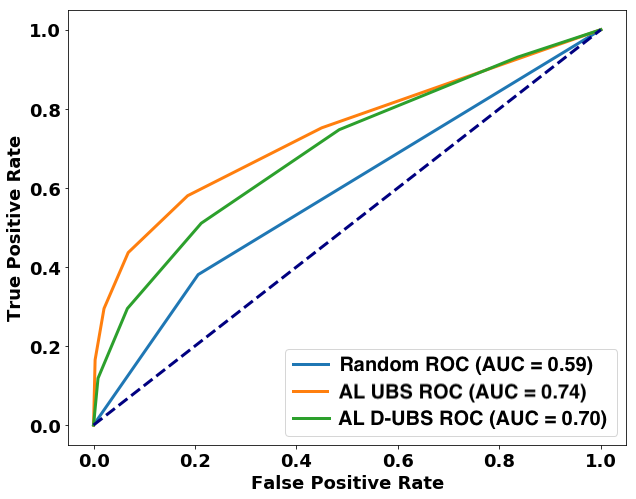
\includegraphics[trim=0in 0.1in 0.1in 0.in,clip,width=1.0\textwidth]{figures/rocs_round5_new.png}
\captionsetup{labelformat=empty}
%\caption{ROC curve for last round of active learning. 
%\logan{I think we could benefit from easier-to-remember labels than AL1 and AL2. I don't remember which is which. Also why does the file say Round 5 and the text iterating curves? If we say ROC is a worse plot, why even show it?}\roselyne{ROC is not worse but perhaps incomplete}
%\roselyne{There are 5 rounds of labeling but 4 rounds of active learning, it's confusing, with the table this is less confusing, I used to say, round, but changed to iteration, will use last. Agreed about the names, but hard to compress these names. I've tried and changed them but they haven't changed in the figure yet.}
%}
\label{fig:rocs_round5}
\end{minipage}\qquad
\hspace{2ex}
\begin{minipage}[b]{.4\textwidth}
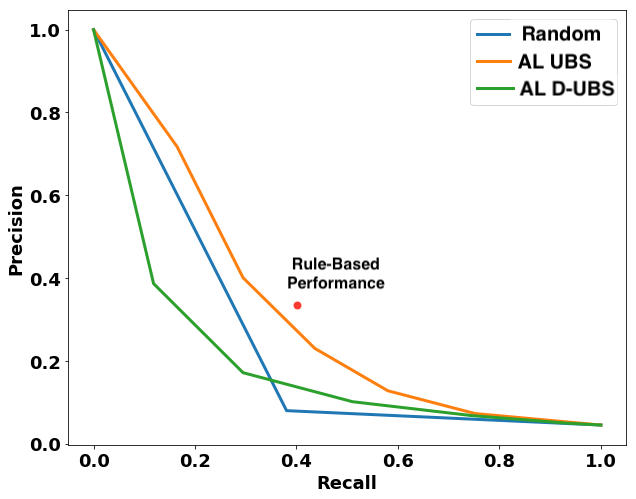
\includegraphics[trim=0in 0.1in 0.1in 0.in,clip,width=1.0\textwidth]{figures/prcs_round5_rule.png}
\captionsetup{labelformat=empty}
%\caption{PR curves for last round of active learning.}
\label{fig:prcs_round5}
\end{minipage}
\setcounter{figure}{8}  
\caption{ROC (left) and PR (right) curves for last round of active learning. 
ROC curves improved from the initial round: AUCs for active learning are 0.74 and 0.7 compared to initial 0.62. 
The classifier based on random sampling does not indicate learning based on AUC. PR curves also show improvement over initial poor performance,
the random strategy has only shows two probabilities for target and non-targets predictions; the other two active learning strategies are lifting away from the bottom corner and indicating discriminative capacities.
In both types of plots, active learning using NLP-filtered candidates (AL UBS) outperforms the active learning using distance candidates (AL D-UBS) and approaches rule-based performance.
% AL-1 refers to active learning using NLP-filtered nouns. AL-2 refers to active learning using candidates deemed similar to representative entities.  %\logan{<soapbox>Is it standard practice to use such uninformativ figure captions in CS? I was taught to make the captions almost standalone from the text</soapbox>}
}\label{fig:rocs_prcs_round5}
\end{figure*}

\subsubsection{Discrimination}
After the initial round of labeling, we experiment with the three strategies mentioned in Section~\ref{sect:apner_architecture}: random sampling (Random), active learning using pool of NLP-filtered nouns from training corpus (UBS), and active learning using pool of \num{10000} distance candidates deemed closest to our seed entities(Distance UBS) \textemdash minus 200 used in initial round).
Given the relatively small batch size, we see no improvement in the PR curve for two rounds of active learning or the first three rounds of labeling. 
Precision remains under 5\% across all used classifiers as shown in Table~\ref{tab:pr_table}. 
%\logan{I think the table would be better suited as a plot}\roselyne{I am tempted to remove it, and just indicate that there was not much learning in the first 3 rounds, but Kyle had a comment that people like to see it for themselves and suggested a table. I don't think the plots would look good either has it will bring attention to the problem of using multiple classifiers as previously discussed. I can go back to ommitting this or displaying the last two rounds.}
%\loganfussingaboutrecallandprecision \roselyne{I actually read that this is what people use many times for imbalanced datasets, but I get the point and we have ROCS to got with the last two rounds}

\begin{table}[ht!]
\centering
\caption{Precision and recall when tested against ground truth documents for classifiers at each active learning round.\label{tab:pr_table}
}
\vspace{2ex}
%[35.55, 37.69, 46.9, 47.97, 46.47, 48.39, 46.68, 36.4]
\setlength\tabcolsep{4pt}
%\begin{tabular}{*4c}
\begin{tabular}{|c|c|c|c|c|}
\hline
& & \multicolumn{3}{c|}{\textbf{Strategies}} \\
 \textbf{Round \#} & \textbf{Metric} & \textbf{Random} & \textbf{UBS}  & \textbf{Distance UBS}  \\
%\hline
%Round 0\ \ & \multicolumn{3}{c|}{} \\
\hline
0 & Precision &        \multicolumn{3}{c|}{6.53\%} \\
0 & Recall\ \ \ \ \ &               \multicolumn{3}{c|}{19.1\%} \\
%\hline
%Round 1\ \  & \multicolumn{3}{c|}{} \\
\hline
1 & Precision     & 3.75\%       &      3.18\%      &  5.28\% \\
1 & Recall\ \ \ \ \ & 0.29\%      &   93.62\%     &  56.81\% \\
%\hline
%Round 2\ \  & \multicolumn{3}{c|}{} \\
\hline
2& Precision      & 1.49\%           &      3.79\%      &  5.35\% \\
2& Recall\ \ \ \ \ & 1.45\%           &    46.38\%      &  10.14\% \\
%\hline
%Round 3\ \  & \multicolumn{3}{c|}{} \\
\hline
3 & Precision      & 6.02\%              &    21.23\%      &  3.93\% \\
3 & Recall\ \ \ \ \ & 44.64\%            &    40.00\%      &  84.35\%  \\
%\hline
%Round 4\ \  & \multicolumn{3}{c|}{} \\
\hline
4& Precision     & 7.06\%          &    18.21\%      &  7.20\% \\
4& Recall\ \ \ \ \ & 40.70\%         &     45.64\%     &  51.88\% \\
\hline
\end{tabular}
\end{table}


However in the third iteration of active learning, we notice an increase in precision in UBS (see Table~\ref{tab:pr_table}). 
This learning is sustained in the following iteration as illustrated on Figures~\ref{fig:rocs_prcs_round5}. 
The AUC for UBS is 0.74 and that of Distance UBS is 0.70. 
The PRCs for both are improved (lifting away from the lower left corner of the graph) over the first round with active learning with UBS showing better tradeoff than with Distance UBS and Random strategies.
%After round 3 and 4, we observe and confirm some, albeit moderate, level context-based predictive ability.
%We also determine that the classifier, which uses UBS is performing better than with the two other strategies.
When tested against our gold standard of 467 one-word polymer names the KNN classifier achieves 18.21\% precision and  45.64\% recall. 
While the candidate generation helps insure that the classes are balanced in the initial batch of labels, using a pool of distance candidates (Distance UBS) does not yield better results than using active learning with a pool of all NLP-filtered candidates (UBS).
Intuitively, basic UBS is able to find \textit{useful} instances (target and non-targets) to be labeled from the entire word embedding space, while examples from Distance UBS are clustered around the seed entities which may be colocated in that space.
We selected seed entities based on their frequency in our corpus, and the yield of target entities during the candidate generation.
Instead, this observation suggests that we could also study how the choice of seed entities impact of the performance of the classifier during the active learning process. 
We revisit this concept of \textit{diversity} of labels in more details in the Section~\ref{sec:discussion}. 
It is worth noting that with limited training data and based solely on context, the classifiers retrieves 45.64\% (more than one third) of the gold standard polymers with a precision of 18.21\%; this after about five hours of expert labeling. 
For comparison, an attempt to extract polymer names using the rule: \textit{if the name contains ``poly'' extract it as a polymer}, would score a precision of 34\% and a recall of 41\% on the same dataset.
We conclude that with our relatively small dataset, we are able to achieve close to rule-based performance, using active learning and minimal amount of labeling (under 5 hours).
%\logan{I think we should show this point on the plot for context. Also, state what you conclude from the comparison. Don't leave it up to the reader to state the conclusion.}

\subsection{Using Active Learning Labels with Character-Level Enhanced Embeddings}
Having used just 1000 labels or 5 hours of expert labeling, the context-based classifier using active learning and a pool of NLP-filtered candidates reached numbers comparable to rule-based performance, but not quite the performance obtained by our reference of state-of-the-art chemistry-aware NLP-toolkit.
Next, we train a word embedding model enhanced with sub-word information using polyNER's labels. 
%\logan{Why are you doing this? You need some motivation for this section, otherwise it kinds of jumps out of nowhere and begs the question: Why did you not use this through the entire study? Maybe you can say this section is devoted to "further tuning the model now that you have a large-enough pool of data to make selections statistically-reasonable"?}
We compare the performance to a state-of-the-art chemistry-aware NLP toolkit. %and we end with a discussion of the results.
FastText uses word representations enriched with character-level information.
This word embedding method considers sub-word information as well as
context, allowing it to consider word morphology differences, such as prefixes
and suffixes. Sub-word information is especially useful for words for which
context information is lacking, as words can still be compared to morphologically similar
existing words. We set the length of the sub-word used for comparison\textemdash
FastText's n_gram parameter\textemdash to five characters, based on our intuition that
many polymers begin with the prefixes ``poly'' or ``poly(.'' 
Therefore, we generate a FastText word embedding model, and generate character-enhanced vectors for our UBS-labeled candidates.


Next, we train a KNN classifier using vectors for these candidates labeled through active learning using a pool of NLP-filtered candidates (identified as best-performing in previous experiments).
%\logan{Confusing. Is UBS not active learning?}\roselyne{it's the sampling method}
We test the classifier against NLP-filtered nouns from our 100-document test set.
The KNN classifier performance improves when using these word vectors as shown in Figure%\ref{fig:UBS_rocs_fasttext} and
~\ref{fig:UBS_prcs_fasttext}.
%\logan{Why sow both figures if you say PRC is better.}\roselyne{I will end up taking them off, as I'm now at 12 pages}
In this case, the classifier achieves 29.7\% precision and 81.9\% recall. 
These numbers are comparable to those achieved by ChemDataExtractor (CDE), a state-of-the-art chemical NLP tool.
As CDE aims to extract all
chemical compounds, not just polymers, it serves only as a demonstration of an
alternative approach in the absence of a polymer NER system (Note that CDE also extracts properties). 
Its recall is high
at 74.5\% but its precision is, as expected, low at 8.7\%. 
%\loganfussingaboutrecallandprecision \roselyne{comes with PRC so should be good here}
We have previously modified CDE with
manually defined polymer identification rules~\cite{tchoua2017towards},
and our polymer-enhanced version of the software (CDE+) achieved 42.2\% precision and 68.3\% recall on the same test set. 
We achieve higher recall than CDE and CDE+ using labels from UBS and FastText vectors and intermediate precision with only $\sim$ five hours of expert labeling.

\subsection{Discussion and Future Work}
\label{sec:discussion}
\roselyne{Add results here, bootstrapping helps enriching dataset, but active learning with distance does not learn faster, it is still better than random. Add that 200 is not enough for a batch size to learn, maybe start with 600? Add that I wouldn't use multiple classifiers. Seed entities do help because AL2 still outperforms random.
Also talk about cross checking here somehow since i do not have enough to have a labeling section for results
Each expert annotates one strategy but we perform crosschecking for 10\% of the first batch of labels to get a measure of agreement between experts.} 
%We confirm agreement between labels for all but 1 of the set of 20 candidates or an agreement of 95\%.}
%\logan{The discussion starts out with your last part of the Results section, skipping over anything else you learned. }
We attribute the increased performance to the character embedding enhancement, which not only recognizes ``poly'' (and yields more names based on this n-gram comparison), but also filters out more anomalous candidates (preceding or following polymer names) generated during tokenization and missed by the filtering steps such as ``\textit{$A_mB_n$}'', or ``\textit{Mw/Mn=1.36}''.  
In other words, the classifiers of character and (context-based) word embedding vectors performs better than classifiers of only context-based word embedding.
Given this result, one may wonder whether the active learning process itself could benefit from using this enhanced vector embedding. 
We repeated the active learning experiment using the entire corpus of NLP-filtered candidates and classifying FastText (enhanced) vectors instead of Gensim vectors at each iteration. 
The classifier's ROC curve did not achieve CDE performance after 5 iterations and was below random performance.%\logan{Wasn't it also worse than the randomly-selected words?}\roselyne{yes, but doesn't it make you want to see another figure more}
These results suggest that the character-level information enhances the classifier's performance only once a certain threshold of context information has been captured by the embedding.
In FastText, the portion of the word embedding vector generated using context varies depending on how much context is available in the entire corpus. 
For words deemed to have \textit{enough} context, vectors do not include any character-level information. 
At the other extreme, for previously unseen words, the embedding is generated solely based on character n-gram information and comparison to other words in the corpus.
During the active learning process, candidates to be labeled by experts are selected using maximum-entropy based uncertainty sampling (for which the prediction probability is the same for both classes, target and non target);
these are also more likely to be candidates which lack context and for which vectors have been generated using character-level information. 
As a result, the expert is presented with several nearly identical candidates (e.g. \textit{PS13k/PMMA12k}, \textit{PS214k/PMMA12k}, and \textit{PS31.6k/PMMA12k}) hindering the learning process as they are located in close vicinity in terms of the full (character and context) word embedding space.
In other words, in this full space, while their uncertainty measure is comparable, these examples are not \textit{diverse}, where diversity is a measure of the distance of the examples to each other or previously labeled instances~\cite{brinker2003incorporating}.
One solution to explore in the future, would be to impose a diversity constraint on the candidates using batch active learning for example~\cite{settles2009active}.
%\logan{There are batch active learning papers, and surely a review. Cite one so that people do not think you're planning to reinvent such methods.}\roselyne{Definitely planned on adding citation but hadn't reread that part, thanks}
%\logan{This seem more like a "Future Work/Can we do even better!?" section than an actual discussion. Should we rename the section accordingly}


%\begin{figure}[H]
\begin{figure}
\centering
%\begin{minipage}[b]{.4\textwidth}
%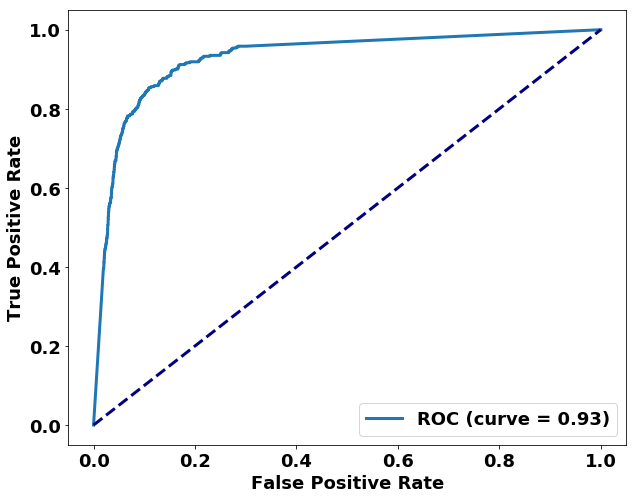
\includegraphics[trim=0in 0.1in 0.1in 0.in,clip,width=3.5in]{figures/fasttext_roc_al_corpus_round5_100}
%\caption{ROC curve for KNN model trained using active learning labels and word representations enriched with character-level information.}\label{fig:UBS_rocs_fasttext}
%\end{minipage}\qquad
%\begin{minipage}[b]{.4\textwidth}
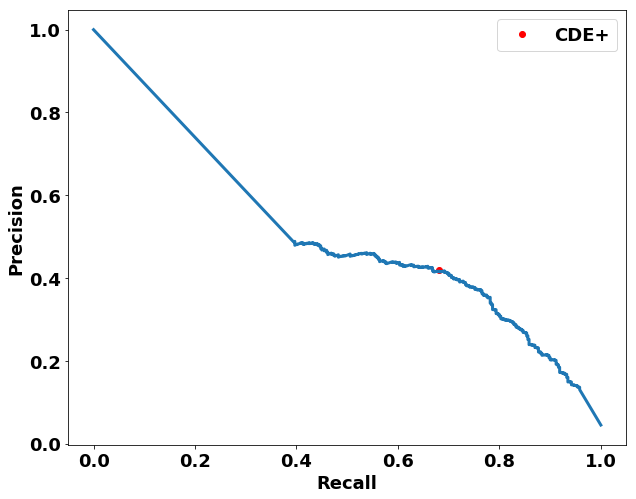
\includegraphics[trim=0in 0.1in 0.1in 0.in,clip,width=3.5in]{figures/fasttext_prc_al_corpus_round5_100}
\caption{PR curve for KNN model trained using active learning labels and word representations enriched with character-level information.}\label{fig:UBS_prcs_fasttext}
%\end{minipage}
\end{figure}











